\documentclass[a4paper, 11pt, compsoc]{IEEEtran}

\usepackage{amsmath}
\usepackage{physics}
\usepackage{hyperref}
\usepackage{cleveref}
\hypersetup{
	colorlinks = true,
	linkcolor = blue,
	filecolor = blue,
	citecolor = black,
	urlcolor = cyan,
}
\crefname{appsec}{Appendix}{Appendices}

\usepackage{graphicx}
\usepackage[section]{placeins}
\usepackage{bookmark}
\usepackage{gensymb}


%for code(MATLAB in particular)
\usepackage{listings}
\usepackage{color} %red, green, blue, yellow, cyan, magenta, black, white
\definecolor{mygreen}{RGB}{28,172,0} % color values Red, Green, Blue
\definecolor{mylilas}{RGB}{170,55,241}

\lstset{
    language=Matlab,%
    %basicstyle=\color{red},
    breaklines=true,%
    morekeywords={matlab2tikz},
    keywordstyle=\color{blue},%
    morekeywords=[2]{1}, 
    keywordstyle=[2]{\color{black}},
    identifierstyle=\color{black},%
    stringstyle=\color{mylilas},
    commentstyle=\color{mygreen},%
    showstringspaces=false,%without this there will be a symbol in the places where there is a space
    numbers=left,%
    numberstyle={\tiny \color{black}},% size of the numbers
    numbersep=7pt, % this defines how far the numbers are from the text
    emph=[1]{for,end,break},
    emphstyle=[1]\color{red}, %some words to emphasise
    %emph=[2]{word1,word2}, emphstyle=[2]{style},
}


\graphicspath{{./pictures/}}

\title{ECEN315 - Compensating a Propeller Driven Pendulum }
\author{Joshua Benfell - 300433229}

\IEEEtitleabstractindextext{
    \begin{abstract}
    \end{abstract}
}


\begin{document}
    \maketitle
    \IEEEdisplaynontitleabstractindextext

    \section{Introduction}\label{sec:intro}
		In the previous report the open loop transfer function was derived for a propeller driven pendulum. The response of the system was stable with oscillations making it unideal for practical use. To improve the system, a compensator will be designed for it to speed up the systems response and make it less oscillatory. To do this, a variety of compensators will be modelled using the simulink package to gain a better understanding of the function and benefits of them. Finally a PID compensator will be implemented with that reduces the settling time of the system at least threefold.
	\section{Background}\label{sec:bg}
	\section{Simulink Model}\label{sec:model}
		\begin{figure}[!ht]
			\centering
			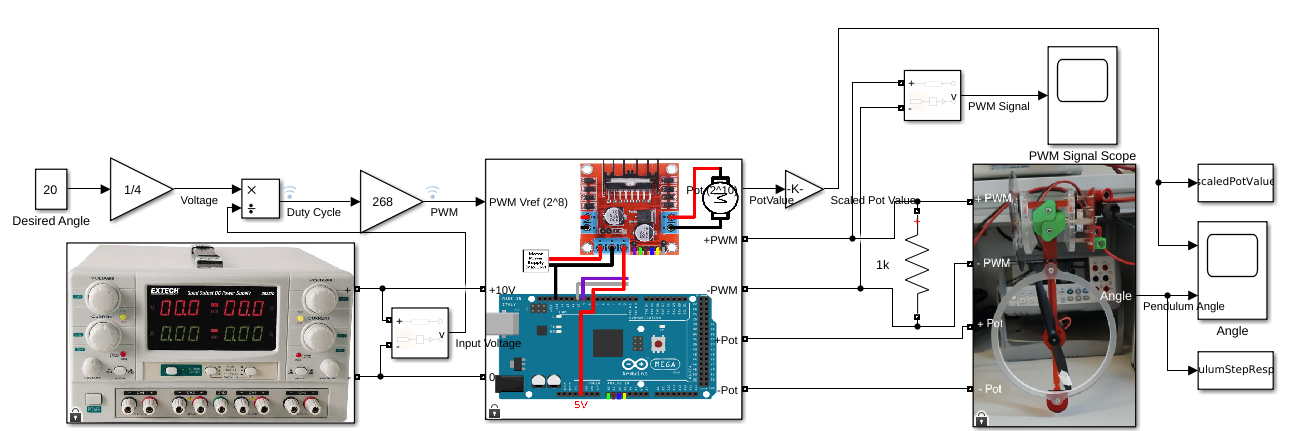
\includegraphics[width=\columnwidth]{lab4System.png}
			\caption{Calibrated Open Loop System}
			\label{fig:baseSystem}
		\end{figure}
		In the last report, the transfer function of our system was derived, however, the derived system is not always an accurate representation of how the actual system will behave. To imitate this dissonant behavior, a slightly different system will be used in the simulink models. The system used in this report (shown in \Cref{fig:baseSystem}, where it is fully calibrated.), takes a PWM reference and then outputs the resultant angular displacement. However, it is desirable that the input units are the same as the output units, so the system needs to be calibrated.
		\par
		There are 3 main calibration stages on the input sides:
		\begin{itemize}
			\item Converting the desired angular displacement into the required applied voltage.
			\item Converting that voltage into a duty cycle
			\item Converting that duty cycle into the PWM value the arduino should output to the motor
		\end{itemize}
		To calibrate these values first start with the angle. By applying a voltage over the pendulum motor an angular displacement can be generated. By applying different voltages, a relationship can be determined between the voltage and the angle. For this system it was found that the voltage required is 4 times less than the desired angle (\Cref{app:calibration}).
		\par
		\begin{figure}[!ht]
			\centering
			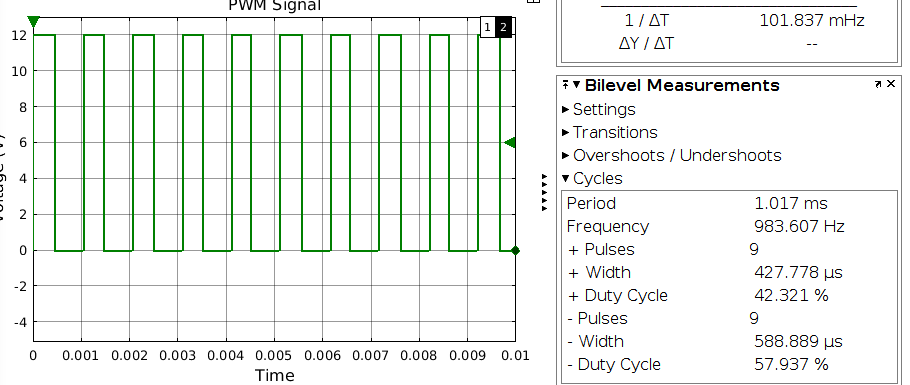
\includegraphics[width=\columnwidth]{dutyCycleSignal.png}
			\caption{Signal Generated by the Arduino}
			\label{fig:signal}
		\end{figure}
		The next constant to determine is the conversion between voltage and a duty cycle. To do this, the system incorporates the arduino to control the effective voltage applied to the motor. A series of PWM values are input into the arduino and the resultant signal will be read across a $1k\Omega$ load, were the duty cycle can be measured (\Cref{fig:signal}). Plotting the relationship between duty cycle and PWM and voltage and duty cycle result in the constants 2.68 and 1/12 respectively (\Cref{app:calibration}); this second constant is 1 over the source voltage. A factor of 100 needs to be added in somewhere along this cascaded chain as the duty cycle is shown as a percentage not a proportion.
		\par
		With the above constants computed, the pendulum will now rise to the desired angle. There is one final constant to compute, and that is the constant to convert the analog potentiometer value into an angle so that the angle can be read for later application; practically the arduino is unable to read the angular displacement without a component such as a potentiometer. To calibrate this constant, the potentiometers value is plotted against the resulting angle; the constant that converts the ADC value to an angle is 1/25 (\Cref{app:calibration}).
		\begin{figure}[!ht]
			\centering
			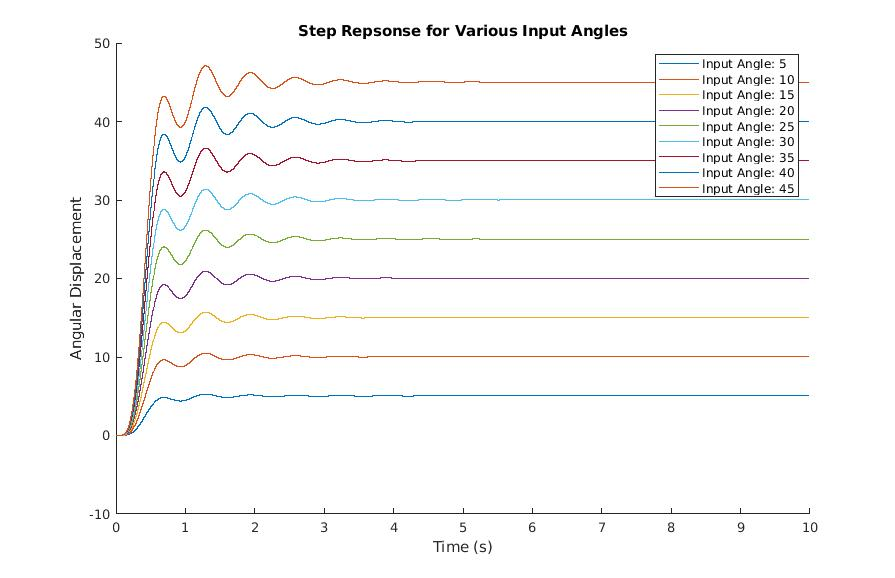
\includegraphics[width=\columnwidth]{lab4Input.jpg}
			\caption{System Response to various desired angles}
			\label{fig:lab4Output}
		\end{figure}
		\begin{figure}[!ht]
			\centering
			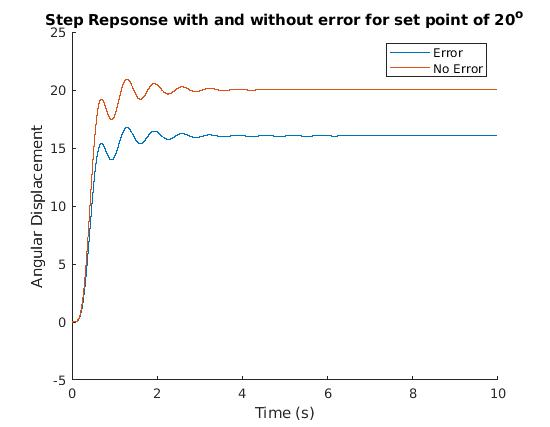
\includegraphics[width=\columnwidth]{lab4Error.jpg}
			\caption{System Response with and without a simulated Error}
			\label{fig:lab4Error}
		\end{figure}
		Finally, the calibrated system needs to be tested to confirm that it reaches the desired input. \Cref{fig:lab4Output} shows the output to various desired inputs, and it can be seen that the system has zero steady state error for all the inputs. However, not all systems are perfect and as such we are able to simulate an error \cref{figlab4Error}. The relation between the error and the steady state value for the system with simulated error is that the error is $0.2 \text{\times steady state value}$, so to account for this, we need to have a gain of 1.25 on the input angle (as the steady state value will be 0.8 the input angle) \cref{app:calibration}. This is not an ideal solution to deal with the error as this requires a different gain value if a different error exist, and this may not be linear. 
    \section{Compensators}\label{sec:comp}
        \subsection{Proportional}\label{sec:p}
        \subsection{PI}\label{sec:pi}
        \subsection{PD}\label{sec:pd}
        \subsection{PID}\label{sec:pid}
    \section{Discussion}\label{sec:disc}
    \section{Conclusion}\label{sec:conc}

    % \Urlmuskip=0mu plus 1mu\relax
    % \bibliography{bibliography}
    % \bibliographystyle{IEEEtran}

    \onecolumn
	\appendices
		\crefalias{section}{appsec}
		\section{Lab 4 Calibration} \label{app:calibration}
			\begin{figure}[!ht]
				\centering
				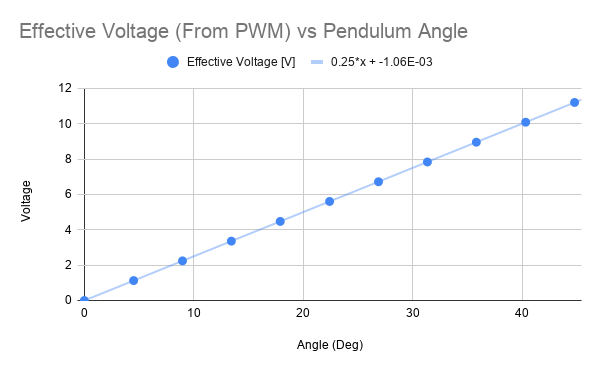
\includegraphics[width=0.8\columnwidth]{angleVoltage.png}
				\caption{Plot of Voltage applied to motor and the angular displacement produced}
				\label{fig:voltAngle}
			\end{figure}

			\begin{figure}[!ht]
				\centering
				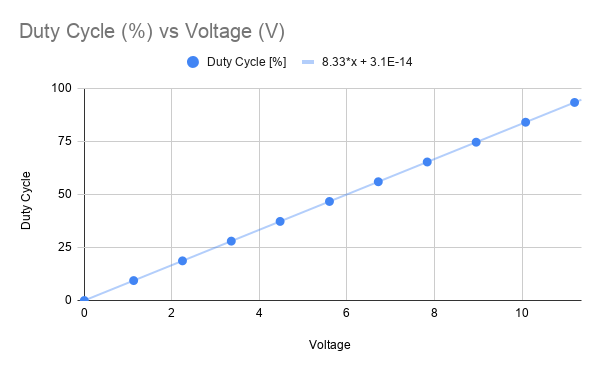
\includegraphics[width=0.8\columnwidth]{dutyCycleVoltage.png}
				\caption{Plot of effective voltage for a given duty cycle}
				\label{fig:DCV}
			\end{figure}

			\begin{figure}[!ht]
				\centering
				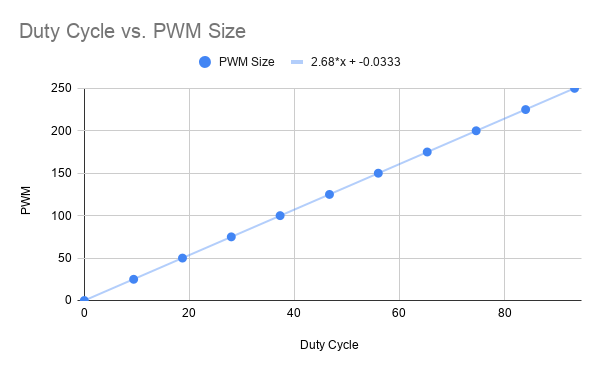
\includegraphics[width=0.8\columnwidth]{dutyCyclePWM.png}
				\caption{Plot of the Duty Cycle that a PWM value creates}
				\label{fig:DCPWM}
			\end{figure}

			\begin{figure}[!ht]
				\centering
				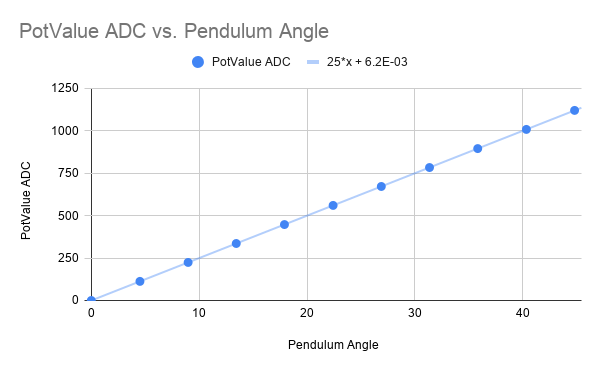
\includegraphics[width=0.8\columnwidth]{potPen.png}
				\caption{Plot of the potentiometer ADC value that an angular displacement causes.}
				\label{fig:potPen}
			\end{figure}
			
			\begin{figure}[!ht]
				\centering
				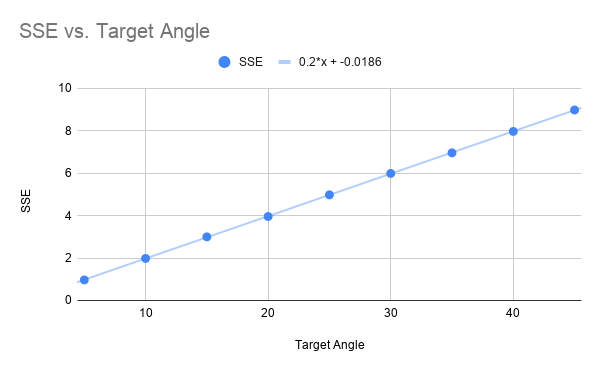
\includegraphics[width=0.8\columnwidth]{lab4SSEvsTarget Angle.png}
				\caption{SSE for a Given input angle when the system has error}
				\label{fig:lab4SSE}
			\end{figure}
\end{document}